\chapter{Kimia Heterosiklik}\label{ch:b3:heterocycles}

Secangkir kopi memuat kafeina, yang tersusun dari dua cincin terpadu yang mengandung empat
atom nitrogen, dan aromanya berasal dari puluhan furan, pirola, pirazina,
dan tiofena yang terbentuk selama penyangraian. Sebagian besar obat di rak apotek mengandung
paling sedikit satu cincin yang memuat atom nitrogen, oksigen, atau belerang, demikian pula basa-basa
DNA, \omterm{def:b3:bioinorganic:haem}{hem} dan klorofil, serta banyak vitamin. Bab ini menjelaskan bagaimana
sebuah heteroatom dalam cincin aromatik mengubah elektron-elektronnya: heteroatom itu dapat membuat cincin
lebih miskin atau lebih kaya elektron daripada benzena, dan hal itu menentukan di mana dan bagaimana cincin itu bereaksi. Bab ini
ditutup dengan tiga cara klasik untuk membangun cincin semacam itu.

\begin{recall}
Jilid Tahun 2 membahas aromatisitas dan aturan Hückel, arena dan
substitusi aromatik elektrofilik melalui zat antara Wheland, gugus
pengaktif dan pengarah, amina dan kebasaannya, imina, enamina,
tautomer, dan basa nukleat; Jilid Tahun 1 membahas $\mathrm pK_a$, nukleofil,
elektrofil, dan gugus pergi. \Cref{ch:b3:pericyclic} memberikan \omterm{def:b3:pericyclic:families}{penataan ulang
sigmatropik} [3,3].
\end{recall}

\begin{omfigure}
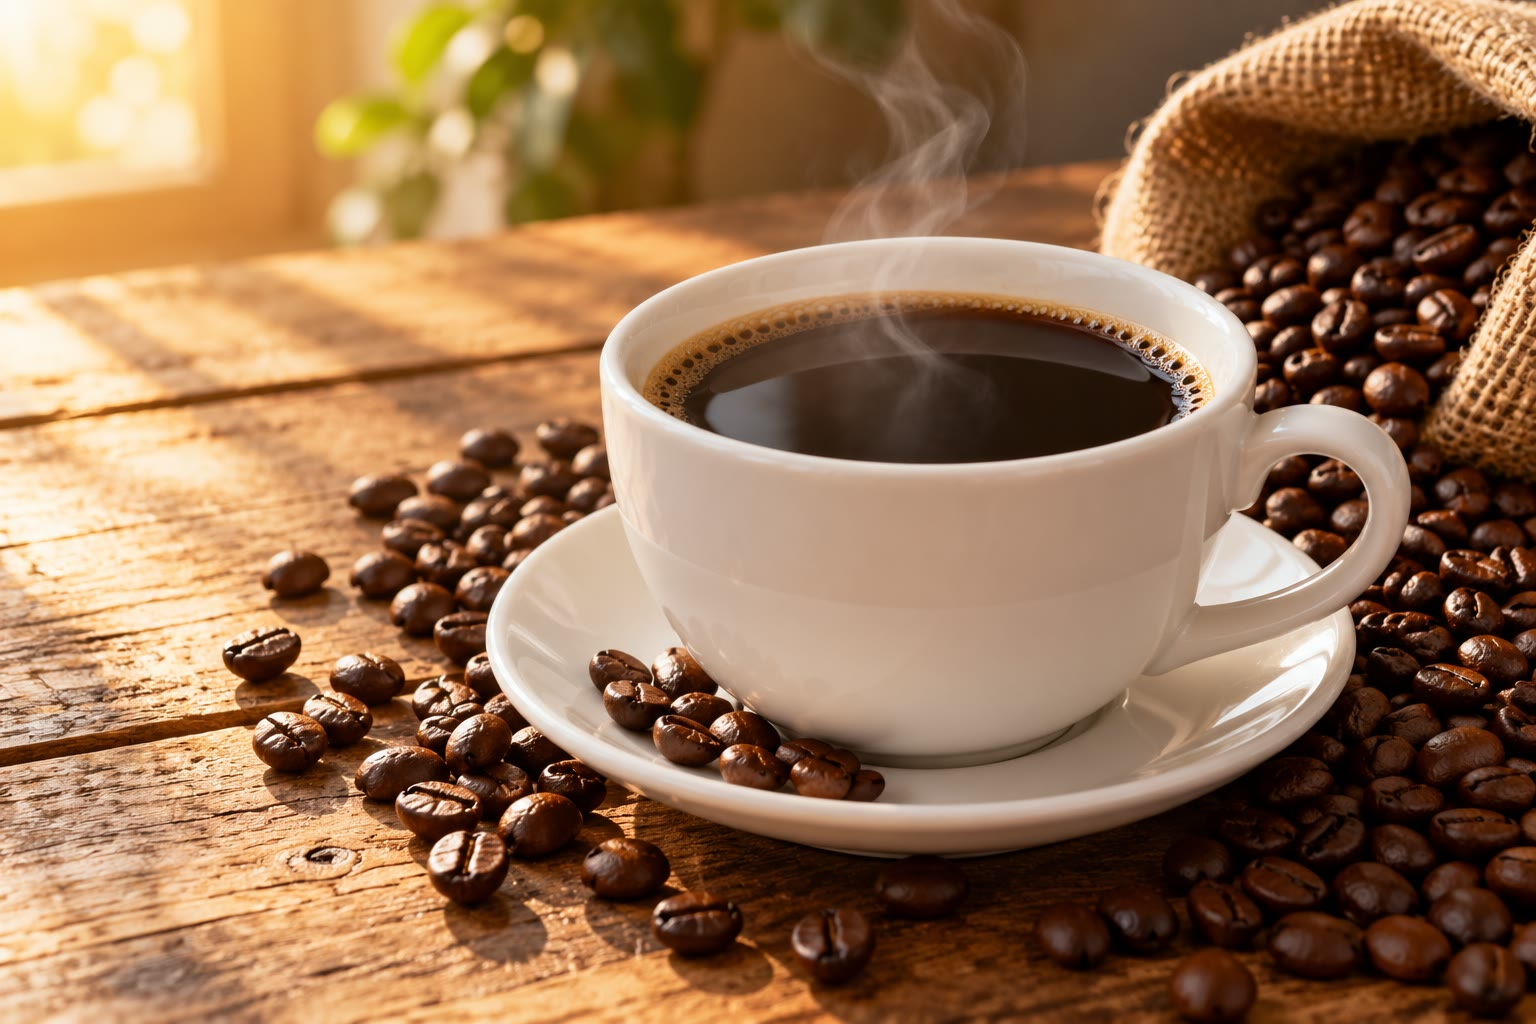
\includegraphics[width=0.5\linewidth]{images/book4/ai/b3-29-coffee.jpg}

{\small Secangkir kopi dan biji yang disangrai: kafeina, sebuah purina, dan banyak
molekul aroma yang terbentuk selama penyangraian merupakan \omterm{def:b3:heterocycles:heterocycle}{heterosiklus}.}
\end{omfigure}

\section{Heterosiklus aromatik}

\begin{definition}[Heterosiklus]\label{def:b3:heterocycles:heterocycle}
Yang disebut \emph{heterosiklus}\index{heterosiklus} adalah senyawa cincin yang memiliki paling sedikit satu
atom selain karbon dalam cincinnya; \emph{senyawa
heteroaromatik}\index{senyawa heteroaromatik} adalah heterosiklus yang aromatik, seperti piridina,
pirola, furan, atau tiofena.
\end{definition}

\begin{proposition}[Enam elektron $\pi$]\label{prop:b3:heterocycles:sextet}
Piridina, pirola, furan, tiofena, dan imidazola masing-masing memiliki enam elektron $\pi$ dalam
cincin datar, siklik, dan terkonjugasi, dan bersifat aromatik menurut aturan Hückel.
\end{proposition}

\begin{proof}
Piridina: kelima karbon dan nitrogen masing-masing menyumbang satu elektron p; pasangan elektron bebas
nitrogen berada dalam orbital $sp^2$ di bidang cincin, di luar sistem $\pi$: $5 + 1 = 6$.
Pirola: empat karbon masing-masing menyumbang satu, dan nitrogen, yang terikat pada H di bidang itu,
menempatkan pasangan elektron bebasnya dalam orbital p-nya: $4 + 2 = 6$. Furan dan tiofena: seperti pirola,
heteroatomnya menyumbang salah satu dari kedua pasangan elektron bebasnya (yang lain terletak di bidang). Imidazola:
nitrogen N--H menyumbang dua, nitrogen yang mirip piridina satu, dan ketiga karbon
tiga: 6. Enam adalah $4n + 2$ dengan $n = 1$.
\end{proof}

\begin{omfigure}
\begin{tikzpicture}[font=\small, yscale=0.55]
  % piridina: enam orbital p tegak lurus terhadap cincin (digambar lebih dahulu), N pada 0 derajat
  \foreach \a in {0,60,...,300} { \pic at (\a:1.1) {omp={0.62}{90}}; }
  \draw[thick] (0:1.1) -- (60:1.1) -- (120:1.1) -- (180:1.1) -- (240:1.1) -- (300:1.1) -- cycle;
  \node[fill=white, inner sep=0.5pt] at (0:1.1) {N};
  \pic at ($(0:1.1)+(0.2,0)$) {omlobe={0.8}{0}};
  \node[font=\scriptsize, align=center, anchor=north] at (0,-2.4) {piridina: 6 elektron p dari 6 atom;\\ pasangan bebas di bidang (basa)};
  \begin{scope}[xshift=5.4cm]
    \foreach \a in {0,72,144,216,288} { \pic at (\a:1.0) {omp={0.62}{90}}; }
    \draw[thick] (0:1.0) -- (72:1.0) -- (144:1.0) -- (216:1.0) -- (288:1.0) -- cycle;
    \node[fill=white, inner sep=0.5pt] at (0:1.0) {N};
    \draw ($(0:1.0)+(0.18,0)$) -- (0:1.7) node[right, inner sep=0.5pt] {H};
    \node[font=\scriptsize, align=center, anchor=north] at (0,-2.4) {pirola: pasangan bebas N adalah salah satu\\ dari 6 elektron $\pi$ (bukan basa)};
  \end{scope}
\end{tikzpicture}

{\small Sistem $\pi$ piridina dan pirola, dilihat secara miring: satu orbital p per
atom cincin, tegak lurus terhadap cincin. Pada piridina, pasangan elektron bebas nitrogen (cuping di bidang, pada
nitrogen) mengarah ke luar di bidang cincin dan bebas mengikat proton; pada pirola,
nitrogen, yang membawa hidrogen di bidang itu, menyumbangkan pasangan elektron bebasnya kepada
sekstet aromatik.}
\end{omfigure}

\begin{definition}[Heterosiklus kaya $\pi$ dan miskin $\pi$]\label{def:b3:heterocycles:pi-character}
Yang disebut \emph{heterosiklus kaya $\pi$}\index{heterosiklus kaya pi@heterosiklus kaya $\pi$}, seperti
pirola, furan, atau tiofena, adalah \omterm{def:b3:heterocycles:heterocycle}{heterosiklus} yang memiliki enam elektron $\pi$ pada lima atom dan \omterm{def:b3:computational-chemistry:dft}{kerapatan
elektron} $\pi$ pada karbon-karbonnya yang lebih tinggi daripada benzena; sedangkan \emph{heterosiklus miskin
$\pi$}\index{heterosiklus miskin pi@heterosiklus miskin $\pi$}, seperti piridina, memiliki
atom cincin elektronegatif yang menarik kerapatan $\pi$ dari karbon-karbonnya.
\end{definition}

\begin{proposition}[Kebasaan]\label{prop:b3:heterocycles:basicity}
Piridina adalah basa sedang dan pirola hampir tidak basa sama sekali; pirola, ketika
terprotonasi dalam asam kuat, menerima proton pada karbon, bukan pada nitrogen.
\end{proposition}

\begin{proof}[Argumen]
% ledger: pka:pyridinium, pka4:pyrrolium, pka4:piperidinium, pka4:imidazolium, pka4:DMAPH
Pasangan elektron bebas piridina berada di luar sistem $\pi$: memprotonasinya tidak mengorbankan
aromatisitas, dan piridinium memiliki $\mathrm pK_a = 5.2$; piridina kurang basa daripada piperidina
(nitrogen piridinium berhibridisasi $sp^2$, dengan karakter s yang lebih besar, dan memegang pasangannya lebih
erat: piperidinium 11.1). Memprotonasi nitrogen pirola akan mengeluarkan pasangan elektron bebasnya
dari sekstet dan merusak aromatisitas; hanya asam yang sangat kuat yang
memprotonasi pirola, yaitu pada C2, tempat kation itu mempertahankan sebagian delokalisasi
($\mathrm pK_a$ sekitar $-4$). Imidazola memiliki kedua jenis nitrogen: imidazola terprotonasi pada
nitrogen yang mirip piridina, dan kationnya, yang simetris, distabilkan oleh resonansi ($\mathrm pK_a$
7.0); itulah sebabnya histidina bekerja sebagai asam dan basa dalam \omterm{def:b3:complex-kinetics:enzyme}{enzim}.
4-(Dimetilamino)piridina lebih basa lagi ($\mathrm pK_a$ 9.6): gugus amino mendorong
pasangan elektron bebasnya ke dalam cincin dan ke nitrogen cincin.
\end{proof}

% ledger: dip:pyridine, dip4:pyrrole, dip4:furan, dip4:thiophene
Momen dipol menceritakan hal yang sama: piridina (\qty{2.19}{D}) memiliki ujung negatifnya
pada nitrogen, sedangkan pada pirola (\qty{1.84}{D}) donasi pasangan elektron bebas ke cincin
menempatkan ujung negatif pada cincin dan ujung positif pada nitrogen. Pada furan
(\qty{0.66}{D}) dan tiofena (\qty{0.55}{D}), kedua efek itu, penarikan $\sigma$ dan donasi $\pi$, hampir
saling meniadakan.

\begin{omfigure}
% ledger: h1:pyridine.a, h1:pyridine.g, h1:pyridine.b, h1:pyrrole.a, h1:pyrrole.b, h1:pyrrole.NH, h1:furan.a, h1:furan.b
\begin{tikzpicture}
\begin{axis}[width=0.86\linewidth, height=6.2cm, x dir=reverse, xmin=5.8, xmax=9.0, ymin=-0.1, ymax=3.6,
  axis x line=bottom, axis y line=none, xlabel={$\delta$ / ppm}, tick label style={font=\scriptsize}, label style={font=\small}]
\addplot[omDef, thick] table[x=ppm, y expr=\thisrow{y}+2.4] {figdata/out/bachelor-3-heterocycle-nmr-pyridine.dat};
\addplot[omThm, thick] table[x=ppm, y expr=\thisrow{y}+1.2] {figdata/out/bachelor-3-heterocycle-nmr-pyrrole.dat};
\addplot[omMeth, thick] table[x=ppm, y=y] {figdata/out/bachelor-3-heterocycle-nmr-furan.dat};
\node[font=\scriptsize, omDef, anchor=west] at (axis cs:7.1,3.0) {piridina: H2/6, H4, H3/5 (2\,:\,1\,:\,2)};
\node[font=\scriptsize, omThm, anchor=west] at (axis cs:7.7,1.8) {pirola: NH, H2/5, H3/4};
\node[font=\scriptsize, omMeth, anchor=west] at (axis cs:7.2,0.6) {furan: H2/5, H3/4};
\end{axis}
\end{tikzpicture}

{\small NMR proton piridina, pirola, dan furan dalam deuterokloroform,
yang disintesis dari geseran terukur sebagai garis-garis tunggal (kopling diabaikan), dengan
luas yang sama dengan jumlah protonnya. Piridina yang miskin $\pi$ memiliki sinyal H2/6 dan H4
jauh di medan bawah sinyal benzena; pirola dan furan yang kaya $\pi$ memiliki sebagian besar
sinyalnya di medan atas sinyal benzena; proton yang bersebelahan dengan heteroatom selalu yang paling
tidak terperisai.}
\end{omfigure}

\section{Piridina}

Piridina menahan substitusi elektrofilik: elektrofil menjumpai cincin yang
lebih miskin elektron daripada benzena, dan, dalam asam yang biasanya hadir, ion
piridinium yang muatan positifnya menolak elektrofil itu. Nitrasi memerlukan kondisi
yang sangat keras dan memberikan isomer-3 dengan rendemen yang buruk.

\begin{proposition}[Substitusi elektrofilik pada C3]\label{prop:b3:heterocycles:pyridine-c3}
Serangan elektrofilik pada piridina terjadi pada C3: serangan pada C2 atau C4 memberikan
zat antara Wheland yang salah satu struktur resonansinya menempatkan muatan
positif pada nitrogen yang hanya dikelilingi enam elektron.
\end{proposition}

\begin{proof}
Pada kation hasil serangan di C2 (atau C4), muatan positif tersebar pada C3, C5,
dan N1 (atau C3, C5, dan N1): sebuah struktur resonansi dengan nitrogen enam elektron yang
kekurangan elektron, yang sangat tidak menguntungkan bagi atom elektronegatif. Serangan
pada C3 menyebarkan muatan hanya pada C2, C4, dan C6. Ketiga kation itu kurang stabil
daripada kation benzena, tetapi serangan pada C3 adalah yang paling tidak buruk.
\end{proof}

\begin{definition}[N-oksida piridina]\label{def:b3:heterocycles:n-oxide}
Yang disebut \emph{N-oksida piridina}\index{N-oksida piridina}, yang dibuat dengan mengoksidasi piridina
dengan asam peroksi, adalah senyawa yang memiliki gugus $\mathrm{N^+{-}O^-}$ yang oksigennya mengembalikan elektron ke C2
dan C4; senyawa itu mengalami substitusi elektrofilik pada C4, dan oksigennya kemudian
disingkirkan.
\end{definition}

\begin{definition}[Substitusi aromatik nukleofilik]\label{def:b3:heterocycles:snar}
Yang disebut \emph{substitusi aromatik nukleofilik}\index{substitusi aromatik nukleofilik}
($\mathrm S_\mathrm NAr$) adalah penggantian gugus pergi pada cincin aromatik yang miskin elektron
oleh sebuah nukleofil, melalui adisi yang diikuti eliminasi. Zat antara adisi yang
anionik itu disebut \emph{kompleks Meisenheimer}\index{kompleks Meisenheimer}.
\end{definition}

\begin{proposition}[$\mathrm S_\mathrm NAr$ pada C2 dan C4]\label{prop:b3:heterocycles:snar-positions}
Halopiridina mudah mengalami $\mathrm S_\mathrm NAr$ pada C2 dan C4 dan hanya lamban pada C3,
karena adisi pada C2 atau C4 menempatkan muatan negatif pada nitrogen.
\end{proposition}

\begin{proof}
Adisi pada C2 membuat C2 berhibridisasi $sp^3$ dan menyisakan empat elektron $\pi$ ditambah pasangan yang masuk
yang tersebar pada N1, C3, dan C5 (atau untuk C4: C3, C5, dan N1): satu struktur resonansi memiliki
muatan negatif pada nitrogen yang elektronegatif. Adisi pada C3 menyebarkannya hanya pada
C2, C4, dan C6, yang semuanya karbon.
\end{proof}

\begin{omfigure}
\begin{tikzpicture}[font=\small, >=Stealth]
  \draw[thick] (-0.000,-0.620) -- (0.537,-0.310) -- (0.537,0.310) -- (0.000,0.620) -- (-0.537,0.310) -- (-0.537,-0.310) -- cycle;
  \draw[thick] (0.082,-0.424) -- (0.326,-0.283);
  \draw[thick] (0.326,0.283) -- (0.082,0.424);
  \draw[thick] (-0.408,0.141) -- (-0.408,-0.141);
  \node[fill=white, inner sep=0.4pt, font=\scriptsize] at (-0.000,-0.620) {N};
  \draw (0.537,-0.310) -- (0.927,-0.535) node[right, inner sep=0.5pt, font=\scriptsize] {Cl};
  \draw[thick] (3.400,-0.620) -- (3.937,-0.310) -- (3.937,0.310) -- (3.400,0.620) -- (2.863,0.310) -- (2.863,-0.310) -- cycle;
  \draw[thick] (3.726,0.283) -- (3.482,0.424);
  \draw[thick] (2.992,0.141) -- (2.992,-0.141);
  \node[fill=white, inner sep=0.4pt, font=\scriptsize] at (3.400,-0.620) {N};
  \node[font=\scriptsize, omThm] at (3.350,-0.920) {$\ominus$};
  \draw (3.937,-0.310) -- (4.386,-0.343) node[right, inner sep=0.5pt, font=\scriptsize] {Nu};
  \draw (3.937,-0.310) -- (4.190,-0.682) node[right, inner sep=0.5pt, font=\scriptsize] {Cl};
  \draw[thick] (6.800,-0.620) -- (7.337,-0.310) -- (7.337,0.310) -- (6.800,0.620) -- (6.263,0.310) -- (6.263,-0.310) -- cycle;
  \draw[thick] (6.882,-0.424) -- (7.126,-0.283);
  \draw[thick] (7.126,0.283) -- (6.882,0.424);
  \draw[thick] (6.392,0.141) -- (6.392,-0.141);
  \node[fill=white, inner sep=0.4pt, font=\scriptsize] at (6.800,-0.620) {N};
  \draw (7.337,-0.310) -- (7.727,-0.535) node[right, inner sep=0.5pt, font=\scriptsize] {Nu};
  \draw[->, thick] (1.25,0) -- (2.35,0) node[midway, above, font=\scriptsize] {$+\,\mathrm{Nu^-}$};
  \draw[->, thick] (4.65,0) -- (5.75,0) node[midway, above, font=\scriptsize] {$-\,\ce{Cl-}$};
  \node[font=\scriptsize] at (3.4,-1.2) {kompleks Meisenheimer};
\end{tikzpicture}

{\small Substitusi nukleofilik 2-kloropiridina: nukleofil teradisi pada
C2, sehingga terbentuk zat antara anionik yang muatan negatifnya sebagian besar berada pada
nitrogen cincin (satu struktur resonansi diperlihatkan); klorida lalu lepas dan
cincin aromatik dipulihkan.}
\end{omfigure}

\begin{proposition}[Adisi--eliminasi]\label{prop:b3:heterocycles:snar-mechanism}
Untuk reaksi $\mathrm S_\mathrm NAr$ yang tahap adisinya menentukan laju, $v = k[\mathrm{ArX}][\mathrm{Nu^-}]$,
dan fluorida adalah gugus pergi halida yang terbaik.
\end{proposition}

\begin{proof}[Argumen]
Lajunya adalah laju adisi bimolekular. Ikatan karbon--halogen tidak
diputus dalam tahap itu; yang penting adalah seberapa jauh halogen menurunkan energi
keadaan transisi anionik dengan menarik elektron, dan fluor, yang paling
elektronegatif, paling kuat melakukannya: urutannya F $>$ Cl $\approx$ Br $>$ I, berlawanan dengan urutan pada $\mathrm S_\mathrm N2$.
\end{proof}

\begin{definition}[Reaksi Chichibabin]\label{def:b3:heterocycles:chichibabin}
Yang disebut \emph{reaksi Chichibabin}\index{reaksi Chichibabin} adalah aminasi
piridina pada C2 oleh natrium amida: ion amida teradisi pada C2, dan sebuah ion hidrida
lepas, sebagai dihidrogen setelah bereaksi dengan produk.
\end{definition}

Piridina dan DMAP juga berfungsi sebagai basa dan sebagai katalis nukleofilik: dalam
asilasi dengan anhidrida asam, DMAP menyerang anhidrida lebih dahulu, sehingga terbentuk
ion asilpiridinium yang memindahkan gugus asilnya ke alkohol jauh lebih cepat daripada
anhidrida itu sendiri. Piridina, bipiridina, dan fenantrolina termasuk
ligan yang paling umum dalam kimia koordinasi.

\section{Cincin beranggota lima}

\begin{proposition}[Substitusi elektrofilik pirola pada C2]\label{prop:b3:heterocycles:pyrrole-c2}
Pirola, furan, dan tiofena mengalami substitusi elektrofilik terutama pada C2,
karena kation hasil serangan pada C2 memiliki tiga struktur resonansi, sedangkan kation
hasil serangan pada C3 hanya dua.
\end{proposition}

\begin{proof}
Setelah serangan pada C2, muatan positif dapat berada pada C3, pada C5, atau pada nitrogen,
tempat muatan itu dibagi melalui pasangan elektron bebas dan setiap atom mempertahankan oktet (struktur
ketiga). Setelah serangan pada C3, muatan itu hanya dapat berada pada C2 atau pada nitrogen: muatannya
kurang terdelokalisasi (lihat gambar).
\end{proof}

\begin{omfigure}
\begin{tikzpicture}[font=\small]
  \draw[thick] (0.000,0.620) -- (0.590,0.192) -- (0.364,-0.502) -- (-0.364,-0.502) -- (-0.590,0.192) -- cycle;
  \draw[thick] (-0.303,-0.269) -- (-0.403,0.039);
  \node[fill=white, inner sep=0.4pt, font=\scriptsize] at (0.000,0.620) {N};
  \draw (0.000,0.750) -- (0.000,1.020) node[above, inner sep=0.5pt, font=\scriptsize] {H};
  \draw (0.590,0.192) -- (0.893,0.482) node[right, inner sep=0.5pt, font=\scriptsize] {H};
  \draw (0.590,0.192) -- (1.006,0.135) node[right, inner sep=0.5pt, font=\scriptsize] {E};
  \node[font=\scriptsize, omThm] at (0.164,-0.226) {$\oplus$};
  \draw[thick] (2.600,0.620) -- (3.190,0.192) -- (2.964,-0.502) -- (2.236,-0.502) -- (2.010,0.192) -- cycle;
  \draw[thick] (2.762,-0.371) -- (2.438,-0.371);
  \node[fill=white, inner sep=0.4pt, font=\scriptsize] at (2.600,0.620) {N};
  \draw (2.600,0.750) -- (2.600,1.020) node[above, inner sep=0.5pt, font=\scriptsize] {H};
  \draw (3.190,0.192) -- (3.493,0.482) node[right, inner sep=0.5pt, font=\scriptsize] {H};
  \draw (3.190,0.192) -- (3.606,0.135) node[right, inner sep=0.5pt, font=\scriptsize] {E};
  \node[font=\scriptsize, omThm] at (2.335,0.086) {$\oplus$};
  \draw[thick] (5.200,0.620) -- (5.790,0.192) -- (5.564,-0.502) -- (4.836,-0.502) -- (4.610,0.192) -- cycle;
  \draw[thick] (5.362,-0.371) -- (5.038,-0.371);
  \draw[thick] (5.113,0.395) -- (4.851,0.205);
  \node[fill=white, inner sep=0.4pt, font=\scriptsize] at (5.200,0.620) {N};
  \draw (5.200,0.750) -- (5.200,1.020) node[above, inner sep=0.5pt, font=\scriptsize] {H};
  \draw (5.790,0.192) -- (6.093,0.482) node[right, inner sep=0.5pt, font=\scriptsize] {H};
  \draw (5.790,0.192) -- (6.206,0.135) node[right, inner sep=0.5pt, font=\scriptsize] {E};
  \node[font=\scriptsize, omThm] at (5.480,0.700) {$\oplus$};
  \draw[thick] (8.400,0.620) -- (8.990,0.192) -- (8.764,-0.502) -- (8.036,-0.502) -- (7.810,0.192) -- cycle;
  \draw[thick] (8.097,-0.269) -- (7.997,0.039);
  \node[fill=white, inner sep=0.4pt, font=\scriptsize] at (8.400,0.620) {N};
  \draw (8.400,0.750) -- (8.400,1.020) node[above, inner sep=0.5pt, font=\scriptsize] {H};
  \draw (8.764,-0.502) -- (9.135,-0.700) node[right, inner sep=0.5pt, font=\scriptsize] {H};
  \draw (8.764,-0.502) -- (8.839,-0.915) node[right, inner sep=0.5pt, font=\scriptsize] {E};
  \node[font=\scriptsize, omThm] at (8.665,0.086) {$\oplus$};
  \draw[thick] (11.000,0.620) -- (11.590,0.192) -- (11.364,-0.502) -- (10.636,-0.502) -- (10.410,0.192) -- cycle;
  \draw[thick] (10.697,-0.269) -- (10.597,0.039);
  \draw[thick] (11.087,0.395) -- (11.349,0.205);
  \node[fill=white, inner sep=0.4pt, font=\scriptsize] at (11.000,0.620) {N};
  \draw (11.000,0.750) -- (11.000,1.020) node[above, inner sep=0.5pt, font=\scriptsize] {H};
  \draw (11.364,-0.502) -- (11.735,-0.700) node[right, inner sep=0.5pt, font=\scriptsize] {H};
  \draw (11.364,-0.502) -- (11.439,-0.915) node[right, inner sep=0.5pt, font=\scriptsize] {E};
  \node[font=\scriptsize, omThm] at (11.280,0.700) {$\oplus$};
  \node[font=\scriptsize] at (2.6,-1.35) {serangan pada C2: tiga struktur};
  \node[font=\scriptsize] at (9.7,-1.35) {serangan pada C3: dua struktur};
  \draw[black!40] (6.8,-1.2) -- (6.8,1.2);
\end{tikzpicture}

{\small Zat antara Wheland pirola (E: elektrofil; $\oplus$: muatan positif).
Serangan pada C2 memberikan kation dengan muatan pada C3, pada C5, atau pada nitrogen dengan semua
oktet lengkap; serangan pada C3, hanya pada C2 atau nitrogen.}
\end{omfigure}

Pirola kira-kira sereaktif fenol atau anilina: pirola dibrominasi, dinitrasi,
dan diasilasi pada kondisi ringan, berpolimerisasi dalam asam kuat, dan
diformilasi pada C2 oleh pereaksi Vilsmeier dari dimetilformamida dan fosforil
klorida. Kereaktifan menurun dengan urutan pirola $>$ furan $>$ tiofena $>$ benzena,
mengikuti kesediaan heteroatom untuk berbagi pasangan elektron bebasnya. Furan,
yang paling tidak aromatik, juga bereaksi sebagai diena dalam reaksi Diels--Alder. Basa
kuat seperti butillitium mendeprotonasi furan dan tiofena pada C2, di samping
heteroatom, sehingga terbentuk pereaksi organolitium.

\begin{method}[Meramalkan tempat serangan pada heterosiklus]\label{met:b3:heterocycles:site}
\begin{enumerate}
  \item Golongkan cincinnya: kaya $\pi$ (heteroatom mirip pirola) atau miskin $\pi$
        (nitrogen mirip piridina).
  \item Elektrofil: pada cincin kaya $\pi$ di C2 (C3 untuk indola, yang serangan pada C2-nya
        akan mengganggu cincin benzena); pada piridina di C3, atau di C4 melalui
        N-oksida.
  \item Nukleofil: pada cincin miskin $\pi$ di C2 atau C4, terutama jika ada gugus pergi
        di sana.
  \item Basa kuat: pada C--H di samping heteroatom.
\end{enumerate}
\end{method}

\section{Heterosiklus terpadu dan heterosiklus biologis}

Indola, yaitu benzena yang terpadu dengan pirola, bereaksi dengan elektrofil pada C3: di sana
zat antaranya mempertahankan cincin benzena tetap utuh, dengan muatan pada nitrogen.
Kuinolina, yaitu benzena yang terpadu dengan piridina, disubstitusi oleh elektrofil pada
cincin benzenanya dan oleh nukleofil pada C2 dan C4. Basa-basa nukleat adalah
pirimidina (sitosina, timina, urasil) dan purina (adenina, guanina), yaitu
pirimidina yang terpadu dengan imidazola. Bentuk okso dan amino-nya (tautomer laktam dan
amina) lebih dominan daripada bentuk hidroksi dan imino, dan hal itu menetapkan pola
donor dan akseptor ikatan hidrogen pada setiap basa, jadi juga pemasangan basa.

\begin{omfigure}
\begin{tikzpicture}[font=\small]
  \node[draw, rounded corners, minimum width=1.8cm, minimum height=2.8cm, fill=omDef!8] at (0,0) {};
  \node[font=\small\bfseries] at (0,1.75) {guanina};
  \node[anchor=east] (g1) at (0.85,0.85) {C6=O};
  \node[anchor=east] (g2) at (0.85,0) {N1--H};
  \node[anchor=east] (g3) at (0.85,-0.85) {C2--N--H};
  \node[draw, rounded corners, minimum width=1.8cm, minimum height=2.8cm, fill=omThm!8] at (3.2,0) {};
  \node[font=\small\bfseries] at (3.2,1.75) {sitosina};
  \node[anchor=west] (c1) at (2.35,0.85) {H--N--C4};
  \node[anchor=west] (c2) at (2.35,0) {N3};
  \node[anchor=west] (c3) at (2.35,-0.85) {O=C2};
  \draw[omMeth, very thick, dotted] (g1.east) -- (c1.west);
  \draw[omMeth, very thick, dotted] (g2.east) -- (c2.west);
  \draw[omMeth, very thick, dotted] (g3.east) -- (c3.west);
\end{tikzpicture}

{\small Pasangan basa guanina--sitosina, skematis: tiga ikatan hidrogen (hijau)
antara oksigen karbonil guanina dan N--H amino sitosina, N1--H
guanina dan N3 cincin sitosina, serta N--H amino guanina dan
oksigen karbonil sitosina. Adenina dan timina membentuk dua.}
\end{omfigure}

\section{Membangun cincin}

\begin{definition}[Sintesis Paal--Knorr]\label{def:b3:heterocycles:paal-knorr}
Yang disebut \emph{sintesis Paal--Knorr}\index{sintesis Paal--Knorr} adalah sintesis yang membuat furan
(dengan asam), pirola (dengan amina primer atau amonia), atau tiofena (dengan
pereaksi belerang) dari senyawa 1,4-dikarbonil.
\end{definition}

\begin{definition}[Sintesis piridina Hantzsch]\label{def:b3:heterocycles:hantzsch}
Yang disebut \emph{sintesis piridina Hantzsch}\index{sintesis piridina Hantzsch} adalah sintesis yang
mengondensasikan aldehida, dua ekuivalen ester $\beta$-keto, dan amonia menjadi
1,4-dihidropiridina, yang dapat dioksidasi menjadi piridina.
\end{definition}

\begin{definition}[Sintesis indola Fischer]\label{def:b3:heterocycles:fischer-indole}
Pada \emph{sintesis indola Fischer}\index{sintesis indola Fischer}, fenilhidrazon
sebuah aldehida atau keton dipanaskan dengan katalis asam: hidrazon itu
bertautomerisasi menjadi ena-hidrazina, yang mengalami \omterm{def:b3:pericyclic:families}{penataan ulang sigmatropik}
[3,3]; siklisasi dan lepasnya amonia memberikan indola.
\end{definition}

\begin{omfigure}
\setchemfig{atom sep=1.8em}
\schemestart
\chemfig{*6(-=-=(-NH-[:30]N=[:-30](-[:-90]CH_3)-[:30]CH_3)-=)}
\arrow{->[$\ce{H+}$][tautomer]}[,1.4]
\chemfig{*6(-=-=(-NH-[:30]NH-[:-30](=[:-90]CH_2)-[:30]CH_3)-=)}
\schemestop
\par\bigskip
\schemestart
\arrow{->[{[3,3]}, lalu][siklisasi, $-\ce{NH3}$]}[,2.2]
\chemfig{*6(-=*5(-=(-CH_3)-N(-H)-)-=-=)}
\schemestop

{\small \omterm{def:b3:heterocycles:fischer-indole}{Sintesis indola Fischer} dari aseton fenilhidrazon. Asam mengubah
hidrazon menjadi tautomer ena-hidrazinanya; penataan ulang [3,3] memutus ikatan
N--N dan membuat ikatan C--C antara karbon cincin yang \textit{orto} terhadap nitrogen dan
$\ce{CH2}$ ujung; amina yang baru menyerang imina, dan lepasnya amonia memberikan
2-metilindola.}
\end{omfigure}

\begin{method}[Mendiskoneksi heterosiklus]\label{met:b3:heterocycles:disconnect}
\begin{enumerate}
  \item Pirola, furan, atau tiofena 2,5-tersubstitusi: diskoneksikan kedua ikatan ke
        heteroatom, kembali ke 1,4-diketon (Paal--Knorr).
  \item 1,4-Dihidropiridina simetris dengan ester pada C3 dan C5: kembali ke satu
        aldehida, dua ester $\beta$-keto, dan amonia (Hantzsch).
  \item Indola 2,3-tersubstitusi: kembali ke fenilhidrazina dan keton
        $\mathrm{R^2CH_2COR^3}$ (Fischer).
  \item Periksalah ketersediaan bagian-bagiannya, lalu regiokimianya jika ketonnya
        tidak simetris.
\end{enumerate}
\end{method}

\begin{definition}[Bioisoster]\label{def:b3:heterocycles:bioisostere}
Yang disebut \emph{bioisoster}\index{bioisoster} adalah gugus yang menggantikan gugus lain dalam
molekul obat sambil mempertahankan aktivitas biologisnya, karena memiliki
ukuran, bentuk, serta pola ikatan hidrogen dan muatan yang serupa, seperti tetrazola sebagai
pengganti asam karboksilat, atau piridina sebagai pengganti cincin benzena.
\end{definition}

\begin{inthelab}[Sebuah pirola Paal--Knorr]
Heksana-2,5-dion, anilina, dan sejumlah katalitik asam 4-toluenasulfonat
dipanaskan dengan refluks dalam toluena di dalam labu yang dilengkapi perangkap Dean--Stark:
air yang terbentuk terbawa sebagai azeotrop dan terkumpul di lengan samping, dan hal itu
mendorong kondensasi sampai tuntas. Jika tidak ada lagi air yang terpisah,
larutan dicuci dengan natrium hidrogenkarbonat berair, dikeringkan, dan diuapkan,
lalu 2,5-dimetil-1-fenilpirola direkristalisasi.
\end{inthelab}

\begin{safety}{\ghs[0.62cm]{GHS02}\ghs[0.62cm]{GHS06}\ghs[0.62cm]{GHS07}\ghs[0.62cm]{GHS08}\ghs[0.62cm]{GHS09}}
% ledger: ghs4:pyridine, ghs4:phenylhydrazine
Piridina: sangat mudah menyala, berbahaya melalui semua jalur paparan, dengan bau yang tajam; dipakai di dalam
lemari asam. Fenilhidrazina: beracun melalui semua jalur paparan, dapat menyebabkan kanker dan cacat
genetik, merusak darah pada paparan berulang, pemeka, sangat beracun bagi
kehidupan akuatik; zat itu ditimbang di dalam lemari asam dengan sarung tangan, dan limbahnya dikumpulkan
secara terpisah.
\end{safety}

\begin{history}[Dua sintesis cincin klasik]
Emil Fischer menguraikan sintesis indolanya pada 1883, pada tahun-tahun yang sama dengan
karyanya tentang gula dan purina; Arthur Hantzsch menerbitkan sintesis piridinanya
pada 1881. Keduanya masih dipakai: sintesis Fischer untuk obat-obat
triptan melawan migrain, sintesis Hantzsch untuk penghambat kanal kalsium
dihidropiridina yang mengobati tekanan darah tinggi.
\end{history}

\section{Latihan}

\begin{exercise}[$\star$]\label{exo:b3:heterocycles:1}
Hitunglah elektron $\pi$ oksazola, tiazola, pirimidina, dan purina, dan sebutkan pasangan elektron bebas
mana yang termasuk dalam sistem $\pi$.
\end{exercise}

\begin{exercise}[$\star$]\label{exo:b3:heterocycles:2}
Urutkan piridina, pirola, imidazola, piperidina, dan DMAP menurut kebasaannya, beserta
nilai $\mathrm pK_a$-nya.
\end{exercise}

\begin{exercise}[$\star$]\label{exo:b3:heterocycles:3}
Berikan produk utama monobrominasi pirola, furan, dan indola.
\end{exercise}

\begin{exercise}[$\star$]\label{exo:b3:heterocycles:4}
Berikan produk reaksi Paal--Knorr heksana-2,5-dion dengan asam saja,
dengan metilamina, dan dengan fosfor pentasulfida.
\end{exercise}

\begin{exercise}[$\star\star$]\label{exo:b3:heterocycles:5}
2-Kloropiridina bereaksi dengan natrium metoksida dalam metanol pada \qty{65}{\celsius}; 3-kloropiridina
hampir tidak bereaksi. Jelaskan, dan berikan produknya.
\end{exercise}

\begin{exercise}[$\star\star$]\label{exo:b3:heterocycles:6}
Berikan produk \omterm{def:b3:heterocycles:chichibabin}{reaksi Chichibabin} piridina dan gambarlah zat antara
adisinya.
\end{exercise}

\begin{exercise}[$\star\star$]\label{exo:b3:heterocycles:7}
\omterm{def:b3:heterocycles:n-oxide}{N-oksida piridina} dinitrasi pada C4. Jelaskan dengan struktur-struktur resonansi, dan sebutkan bagaimana
4-nitropiridina diperoleh.
\end{exercise}

\begin{exercise}[$\star\star$]\label{exo:b3:heterocycles:8}
2-Hidroksipiridina dalam air terutama berupa 2-piridon. Gambarlah kedua tautomer dan
jelaskan mengapa piridon itu tetap aromatik.
\end{exercise}

\begin{exercise}[$\star\star$]\label{exo:b3:heterocycles:9}
Berikan komponen-komponen sintesis Hantzsch untuk 1,4-dihidropiridina dengan
ester metil pada C3 dan C5, gugus metil pada C2 dan C6, dan gugus 2-nitrofenil
pada C4.
\end{exercise}

\begin{exercise}[$\star\star\star$]\label{exo:b3:heterocycles:10}
Butanon memberikan dua indola yang berbeda dalam sintesis Fischer dengan
fenilhidrazina. Berikan keduanya, dan sebutkan bagaimana kekuatan asam mengubah rasionya.
\end{exercise}

\begin{exercise}[$\star\star\star$]\label{exo:b3:heterocycles:11}
Jelaskan mengapa 4-fluoronitrobenzena dan 2-fluoropiridina bereaksi lebih cepat dengan
nukleofil daripada klorida-kloridanya, tidak seperti substrat $\mathrm S_\mathrm N2$.
\end{exercise}

\begin{exercise}[$\star\star\star$]\label{exo:b3:heterocycles:12}
Dengan spektrum-spektrum sintetis bab ini, jelaskan bagaimana piridina,
pirola, dan furan dapat dibedakan melalui NMR proton, dan ramalkan spektrum
tiofena (geseran \qty{7.33}{ppm} dan \qty{7.12}{ppm}).
\end{exercise}

\section{Soal: Membangun Sebuah Indola}

\begin{problem}[{Soal akhir pekan --- membangun sebuah indola: fenilhidrazon
aseton, ena-hidrazina dan penataan ulang [3,3]-nya, lepasnya amonia,
dan pilihan antara dua indola dengan butanon}]
\label{pb:b3:heterocycles:1}
% ledger: aw:C, aw:H, aw:N, aw:O
Data soal: 10.0 g fenilhidrazina bereaksi dengan aseton berlebih, dan
hidrazonnya dipanaskan dengan seng klorida.

\medskip\noindent\textbf{Bagian I --- Hidrazon.}
\begin{enumerate}[beginpenalty=10000]
  \item Tuliskan pembentukan aseton fenilhidrazon.
  \item Mengapa reaksi itu merupakan kondensasi bertipe imina, dan mengapa sesedikit asam berguna?
  \item Nitrogen fenilhidrazina manakah yang menyerang gugus karbonil, dan mengapa?
  \item Hitunglah massa molar fenilhidrazina dan jumlah yang dipakai.
  \item Hitunglah massa teoretis hidrazon.
\end{enumerate}

\medskip\noindent\textbf{Bagian II --- Ena-hidrazina dan tahap [3,3].}
\begin{enumerate}[resume, beginpenalty=10000]
  \item Gambarlah tautomer ena-hidrazinanya.
  \item Keenam atom manakah yang membentuk keadaan transisi siklik penataan ulang [3,3]?
  \item Ikatan manakah yang putus dan ikatan manakah yang terbentuk?
  \item Berapa banyak elektron yang terlibat, dan apakah tahap itu diizinkan secara termal?
  \item Apakah fungsi seng klorida?
  \item Mengapa aromatisitas cincin benzena harus dipulihkan sesudahnya?
\end{enumerate}

\medskip\noindent\textbf{Bagian III --- Menutup cincin.}
\begin{enumerate}[resume, beginpenalty=10000]
  \item Amina manakah yang menyerang karbon manakah untuk menutup cincin beranggota lima?
  \item Molekul kecil apakah yang lepas, dan apakah yang mendorong tahap terakhir?
  \item Tuliskan persamaan keseluruhannya, dari hidrazon menjadi 2-metilindola.
  \item Hitunglah massa molar 2-metilindola.
  \item Hitunglah massa teoretis 2-metilindola.
  \item Di manakah 2-metilindola akan disubstitusi oleh elektrofil, dan mengapa?
\end{enumerate}

\medskip\noindent\textbf{Bagian IV --- Butanon.}
\begin{enumerate}[resume, beginpenalty=10000]
  \item Gambarlah kedua ena-hidrazina butanon fenilhidrazon.
  \item Berikan kedua indola yang dihasilkannya.
  \item Ena-hidrazina manakah yang lebih tersubstitusi, dan manakah yang terbentuk dalam asam kuat?
  \item Indola manakah yang dominan dengan asam lemah, dan mengapa?
  \item Mengapa asetaldehida fenilhidrazon tidak dapat memberikan indola itu sendiri dengan baik?
  \item Apakah arti masalah regiokimia itu bagi sintesis sebuah obat?
  \item Nyatakan hasilnya: massa teoretis 2-metilindola dari 10.0 g
        fenilhidrazina.
\end{enumerate}
\end{problem}
